\chapter{Proxy Adaptativo para Protocolos Web Avanzados}
\label{spdyproxypython}

\section{Introducci'on}

A lo largo de los cap'itulos anteriores, se ha visto, el crecimiento de Internet, en el Cap'itulo \ref{desarrolloWeb}, las deficiencias de los protocolos, en el Cap'itulo \ref{protocolos}, y la problem'atica de los tiempos de carga y sus posibles optimizaciones en el Cap'itulo \ref{problematica}. Tambi'en se ha visto SPDY como propuesta a resolver varios de los problemas actuales de la carga de los sitios, pero tambi'en, en ciertos contextos no funciona como lo esperado (ver Secci'on \ref{estudiosSPDY}).

Por todo ello, se propone, desarrolla y eval'ua un \textit{Proxy Adaptativo}, que selecciona, de los m'etodos habilitados que ofrezca un sitio (HTTP HTTPS, SPDY), cu'al es el 'optimo para recuperar el recurso, en base a informaci'on almacenada de recuperaciones previas. Posee otras funcionalidades tales como, ser MITM\footnote{Man in The Middle.}, cach'e, c'alculo de RTT, recuperaci'on de los m'etodos habilitados para un sitio, cliente SPDY.

Para el desarrollo del proxy, se escogi'o Python\footnote{https://www.python.org/} como lenguaje principal, dada la facilidad del mismo y la gran documentaci'on disponible en la web. Para el almacenamiento de los datos de los sitios se escogi'o MongoDB\footnote{http://http://www.mongodb.org/}, por su simple interacci'on con Python y su alta velocidad.

Todo el c'odigo del trabajo se encuentra alojado en un repositorio de Github\footnote{https://www.github.com}, que es un repositorio para alojar proyectos de c'odigo abierto. El repositorio puede navegarse desde \citep{spdyproxypython}.

\section{Funcionamiento}

El proxy se inicia en una direcci'on y en un puerto, por ejemplo: \textit{localhost:8080} se debe configurar el navegador para que utilice la direcci'on del proxy para conectarse a Internet. Por ejemplo en Google Chrome se puede iniciar con un flag para configurar el proxy:
\begin{quote}
\textit{chrome --proxy-server="localhost:8080"}
\end{quote}
Acepta tanto conexiones HTTP, como HTTPS en el mismo puerto. Al realizar la conexi'on por SSL con el cliente en vez de actuar de ''puente'' con el destino final, utiliza un certificado SSL para realizar la autenticaci'on.

Cuando recibe una petici'on HTTP, el m'etodo que llega al proxy es \textit{GET}, se consulta la cach'e para ver si el recurso se encuentra almacenado para retornarlo desde la copia del proxy, si no se encuentra, se pide al servidor correspondiente y se devuelve el recurso al cliente. Luego, se realiza el an'alisis del recurso (ver \ref{analisisRecurso}) en segundo plano.

Cuando recibe una petici'on HTTPS, el m'etodo que llega al proxy es CONNECT, que es un m'etodo especial para solicitarle a un proxy una conexi'on al servidor final. En este caso, el proxy responde con el mensaje:
\begin{quote}
\textit{\textit{HTTP/1.1 200 Connection established}}
\end{quote}
para indicarle que se va a realizar la conexi'on. Esta primera etapa puede verse en la Figura \ref{mitm1}.

\begin{figure}[h]
  	\centering
	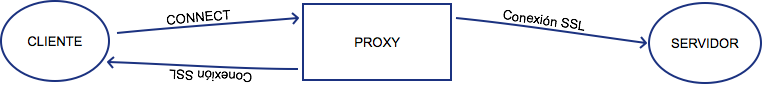
\includegraphics[width=\textwidth]{img/mitm1}
	\caption{\small Conexi'on inicial cuando el protocolo es HTTPS}
	\label{mitm1}
\end{figure}
\vspace{3cm}
Luego, se inicia la conexi'on SSL cliente-proxy y comienzan a recibirse las peticiones del cliente, como puede verse en la Figura \ref{mitm2}, las conexiones\footnote{Tanto hacia el cliente como hacia el Servidor.} se realizan individualmente (no como un t'unel HTTPS normal, ver Figura \ref{proxy_2}). Con cada una de las peticiones, se procede de manera similar a HTTP. Se analiza si el recurso se encuentra almacenado en la cach'e y se devuelve de la copia local, o se solicita el recurso al servidor final. En el caso de que el m'etodo seleccionado para devolver el recurso sea HTTS o SPDY, se establece una conexi'on segura entre el proxy y el servidor final.

\begin{figure}[h]
  	\centering
	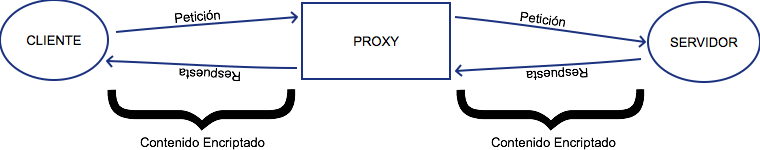
\includegraphics[width=\textwidth]{img/mitm2}
	\caption{\small Procedimiento una vez realizada la conexi'on en los 2 extremos}
	\label{mitm2}
\end{figure}

Cabe destacar que, todo el tr'afico que fluye entre el cliente y el proxy, y entre el proxy y el servidor final, viaja encriptado. Pero, todo el tr'afico se encuentra desencriptado en el proxy, siendo este, un proxy HTTPS de confianza (ver \ref{mitm}, discusi'on en \citep{draftTrustedProxy}).

\subsection{An'alisis de los Recursos}
\label{analisisRecurso}
Cada vez que el proxy recibe una petici'on del cliente, se analiza si el recurso se encuentra en la cach'e, en el caso de que el recurso se encuentre almacenado, se devuelve desde la copia local del proxy y se actualiza la cach'e con el HIT del elemento correspondiente. Caso contrario, se peticiona el recurso servidor final.
Cada vez que el proxy pide un recurso, se realiza un an'alisis del mismo en segundo plano:
\begin{enumerate}
\item C'alculo del tama'no del recurso.
\item C'alculo del RTT: se realiza el c'alculo del RTT al host donde se aloja el recurso.
\item Obtenci'on de Protocolos: se obtienen los protocolos soportados (HTTP, HTTPS, SPDY) del host donde se aloja el recurso.
\item C'alculo de Peticiones a Generar: en el caso de que el recurso sea un HTML plano, se calcula cuantas peticiones generar'ia. Se realiza analizando el texto y extrayendo los recursos que esa p'agina va a necesitar para su renderizaci'on.
\end{enumerate}
Toda esta informaci'on, luego es consumida por un 'arbol de decisi'on para determinar que protocolo es el m'as 'optimo para recuperar el recurso.

\subsection{'Arbol de Decisi'on}

Una vez que se recibe la petici'on del cliente, y hay que peticionar el recurso al servidor final, se decide con qu'e m'etodo se debe traer el recurso. Se tom'o como referencia, el 'arbol de ''How Speedy is SPDY?'' \citep{howSpeedy}, que puede verse en la Figura \ref{arbolDecision}.

\begin{figure}[h]
  	\centering
	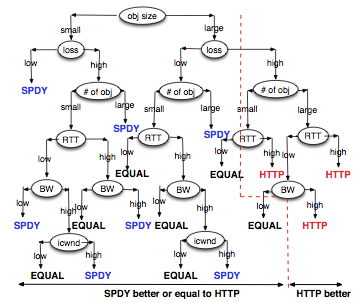
\includegraphics{img/arbolDecision}
	\caption{\small 'Arbol de Decisi'on, extra'ido de \citep{howSpeedy}}
	\label{arbolDecision}
\end{figure}

Este 'arbol, se retroalimenta con la informaci'on que se extrae de los recursos a medida que el proxy est'a en funcionamiento. Datos tales como tama'no, RTT, peticiones a generar, se obtienen del almacenamiento propio del proxy. 

\vspace{4cm}

\section{M'odulos Adicionales}

\subsection{C'alculo del RTT}
\label{measureRTT}
M'odulo que se encarga de realizar un Ping\footnote{Utilidad que comprueba el estado de otro host por medio del env'io de paquetes ICMP de solicitud y de respuesta \citep{ping}.} hacia el host del que se busca obtener la latencia entre ambos nodos. El proxy env'ia un solo paquete ICMP al servidor y se espera su respuesta. Una vez obtenido el resultado, se almacena en la base de datos local.
Tambi'en, ofrece la posibilidad de realizar peticiones masivas, leyendo URLs desde un archivo de texto. Esta opci'on es 'util por ejemplo, para ejecutar antes de iniciar el proxy, y as'i obtener mediciones a priori de hosts que ser'an visitados.

\subsection{Protocolos Habilitados}

M'odulo que se encargar de identificar que protocolos soporta un sitio en cuesti'on. Los protocolos de los que se intenta averiguar si el sitio tiene disponible son HTTP, HTTPS y SPDY. El procedimiento es el siguiente: 
\begin{enumerate}
\item HTTP:
Se intenta realizar una conexi'on al puerto por defecto de HTTP, el puerto 80. En el caso de tener 'exito, se marca HTTP como un protocolo soportado.
\item HTTPS:
Se intenta realizar una conexi'on al puerto por defecto de HTTPS, el puerto 443. En el caso de tener 'exito, se marca HTTPS como un protocolo soportado.
\item SPDY
En el caso de SPDY, se utiliz'o el cliente desarrollado junto con el proxy (ver \ref{clienteSPDY}). Al igual que con los otros protocolos, se intenta realizar una conexi'on segura con el servidor final, si la conexi'on tiene 'exito, se intenta iniciar una sesi'on SPDY con el servidor. Si el inicio de la sesi'on es correcto, se marca SPDY como un protocolo soportado.
\end{enumerate}

Al igual que el m'odulo que calcula el RTT (ver \ref{measureRTT}), 'este posee una opci'on para realizar la verificaci'on de los protocolos habilitados, leyendo un archivo de texto con las URLs. Tal como el m'odulo antes descripto, es 'util para poseer informaci'on previo a la utilizaci'on del proxy.

\subsection{Cliente SPDY}
\label{clienteSPDY}

Python no trae soporte nativo para SPDY, por ello se busc'o una librer'ia que pueda brindar la funcionalidad del protocolo. La seleccionada fue Spdylay \citep{spdylay} de Tatsuhiro Tsujikawa, que, si bien es para el lenguaje C, provee una extensi'on para utilizarla desde Python\footnote{http://tatsuhiro-t.github.io/spdylay/python.html}. Utilizando esta librer'ia, se dise'no un cliente para poder realizar y mantener una sesi'on a trav'es de una conexi'on TCP con un servidor que soporte SPDY. El m'odulo permite iniciar una conexi'on con un servidor y luego iniciar la sesi'on SPDY. Luego, se pueden realizar peticiones a trav'es de la misma conexi'on.